% sections/05_etapa3_colombia.tex
\newcommand{\etapacolombia}{%

\begin{frame}{Dataset: elecciones locales Colombia 2023}
\begin{columns}[c]
\column{0.50\textwidth}
  \textbf{\color{elanGold}Construcción del dataset}
  \begin{itemize}\itemsep0.4em
    \item Universo: 33 ciudades más pobladas
    \item Excluidas: Bogotá (sesgo influencer) + Piedecuesta (sin datos digitales)
    \item Universo final: \textbf{\color{elanGold}31 ciudades competitivas}
    \item Candidatos con $>$10,000 votos: \textbf{\color{elanGold}120 candidatos}
    \item Publicaciones \'unicas: \textbf{\color{elanGold}5,776}
    \begin{itemize}
      \item[\color{elanBlue}·] Facebook: 2,511
      \item[\color{elanBlue}·] Twitter/X: 2,346
      \item[\color{elanBlue}·] TikTok: 919
    \end{itemize}
    \item Ventana de captura: \textbf{14 días} previos a los comicios
    \item Cobertura digital: \textbf{92.6\%} de candidatos con publicaciones activas
  \end{itemize}
\column{0.46\textwidth}
  \begin{tikzpicture}
    \fill[elanPanel] (0,0) rectangle (5.5,5.5);
    \node[anchor=north, yshift=-0.2cm, text=elanGold, font=\bfseries\small] at (2.75,5.5)
      {Pipeline de extracción};
    \node[anchor=north, yshift=-0.9cm, text width=5.0cm] at (2.75,5.5) {
      \small
      \begin{tabular}{ll}
        \color{elanBlue}\textbf{Facebook} & Apify scraper\\
        \color{elanBlue}\textbf{Twitter/X} & Playwright headless\\
        \color{elanBlue}\textbf{TikTok} & API privada (Apify)\\
        \color{elanRed}\textbf{Instagram} & Excluido (API restrictions)\\
      \end{tabular}
    };
    \node[anchor=south, yshift=1.0cm] at (2.75,0) {
      \begin{tikzpicture}
        \fill[elanGold!20!elanPanel] (0,0) rectangle (5.0,1.3);
        \draw[elanGold, line width=0.8pt] (0,0) rectangle (5.0,1.3);
        \node[anchor=center, text=elanGold, font=\bfseries\small] at (2.5,0.95)
          {Reconstrucci\'on Weibull};
        \node[anchor=center, text=elanGray, font=\footnotesize] at (2.5,0.40)
          {aplicada a todas las publicaciones};
      \end{tikzpicture}
    };
  \end{tikzpicture}
\end{columns}
\end{frame}

\begin{frame}{Evidencia descriptiva: dominancia digital y votos}
  \begin{center}
    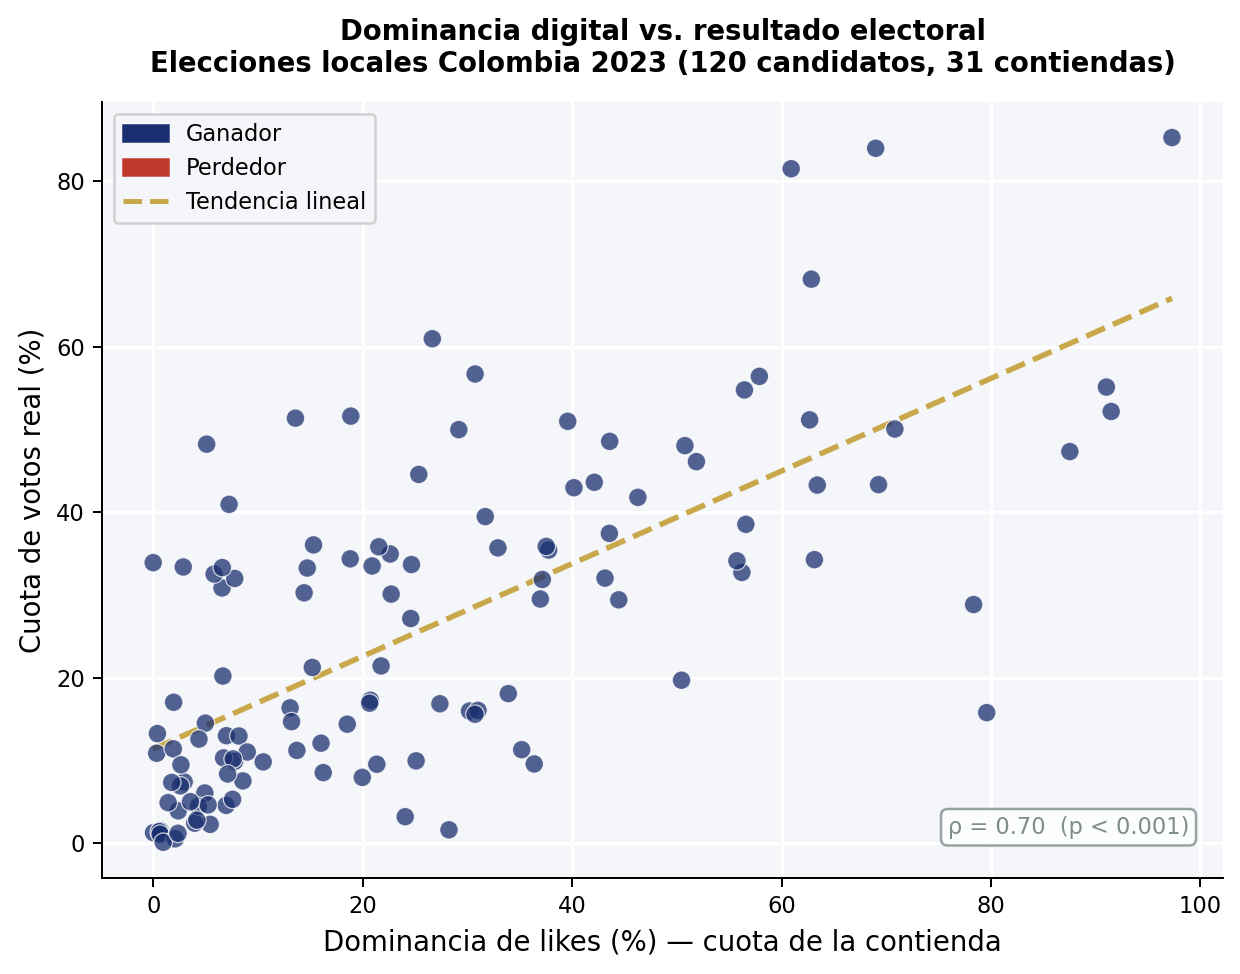
\includegraphics[width=0.78\textwidth]{img/colombia/col_scatter_dominancia_votos.png}
  \end{center}
  \vspace{-0.6em}
  \begin{tikzpicture}
    \fill[elanPanel] (0,0) rectangle (\textwidth,0.75);
    \node[anchor=west, xshift=0.3cm, yshift=0.37cm] at (0,0)
      {{\color{elanGold}\small\bfseries $\rho = 0.70$, $p < 0.001$} \quad
       {\color{elanGray}\small $\cdot$ Ganadores (azul) vs.\ perdedores (rojo) $\cdot$ 120 candidatos, 31 contiendas}};
  \end{tikzpicture}
\end{frame}

\begin{frame}{Modelado predictivo: regresión logística fraccional}
\begin{columns}[c]
\column{0.50\textwidth}
  \textbf{\color{elanGold}Especificaci\'on del modelo}\\[0.4em]
  La variable objetivo es la \textbf{cuota de voto real} $v_c \in (0,1)$.\\[0.5em]
  Dado que $v_c$ es una proporci\'on, usamos regresi\'on log\'{\i}stica fraccional (Papke \& Wooldridge, 1996):
  \[
    \mathbb{E}[v_c \mid X] = \frac{1}{1 + e^{-(\beta_0 + X^\top \beta)}}
  \]
  con predictor central:
  \[
    \text{logit}(\delta_c) = \log\!\left(\frac{\delta_c}{1-\delta_c}\right)
  \]
  \vspace{0.3em}
  \textbf{\color{elanGold}Selección de variables: ElasticNet anidado}\\
  \[
    \hat{\beta} = \arg\min_\beta \bigl\{L(\beta) + \lambda_1\|\beta\|_1 + \lambda_2\|\beta\|_2^2\bigr\}
  \]

\column{0.48\textwidth}
  \textbf{\color{elanGold}Comparativa de modelos}\\[0.2em]
  {\scriptsize M\'etricas LOCO-CV (31 contiendas)}\\[0.1em]
  {\tiny
  \begin{tabular}{@{}lrrr@{}}
    \toprule
    \color{elanWhite} Modelo & \color{elanGold} MAE & \color{elanGold} $R^2$ & \color{elanGold} T1\\
    \midrule
    Base uniforme  & 12.49 & 0.306 & 39\%\\
    Base proporcional & 12.61 & 0.185 & 71\%\\
    Reg. fraccional   & 11.52 & 0.460 & 71\%\\
    \rowcolor{elanPanel}
    \color{elanGold}\bfseries ELA-NOM & \color{elanGold}\bfseries 9.43 & \color{elanGold}\bfseries 0.518 & \color{elanGold}\bfseries 64.5\%\\
    Grad. Boosting    & 9.91 & 0.515 & 67.7\%\\
    \bottomrule
  \end{tabular}}

  \vspace{0.4em}
  \begin{tikzpicture}
    \fill[elanGold!20!elanPanel] (0,0) rectangle (5.5,1.5);
    \draw[elanGold, line width=0.7pt] (0,0) rectangle (5.5,1.5);
    \node[anchor=north, yshift=-0.1cm, text width=5.2cm] at (2.75,1.5) {
      {\color{elanGold}\bfseries\small Validaci\'on: LOCO-CV}\\
      {\color{elanGray}\footnotesize \textit{Leave-One-Contest-Out CV}: en cada pliegue
      se excluye una contienda completa y el modelo predice \textbf{fuera de muestra}.
      31~pliegues $\cdot$ unidad~=~contienda.}
    };
  \end{tikzpicture}
\end{columns}
\end{frame}

\begin{frame}{Coeficientes: estabilidad inter-pliegue (bootstrap)}
  \begin{center}
    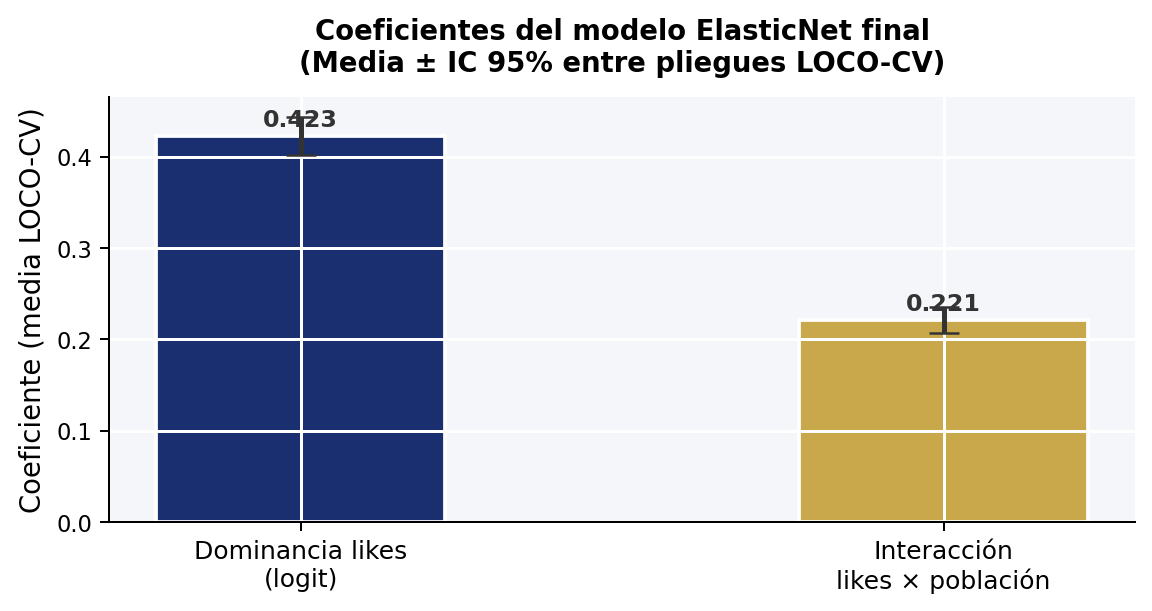
\includegraphics[width=0.82\textwidth]{img/colombia/col_coef_bootstrap.png}
  \end{center}
  \vspace{-0.4em}
  \begin{tikzpicture}
    \fill[elanPanel] (0,0) rectangle (\textwidth,0.75);
    \node[anchor=west, xshift=0.3cm, yshift=0.37cm] at (0,0)
      {{\color{elanGold}\small\bfseries Estabilidad:}
       {\color{elanGray}\small\ logit\_likes e interacción presentes en el 100\% de los pliegues de validación}};
  \end{tikzpicture}
\end{frame}

\begin{frame}{Residuales LOCO-CV: distribución del error}
  \begin{center}
    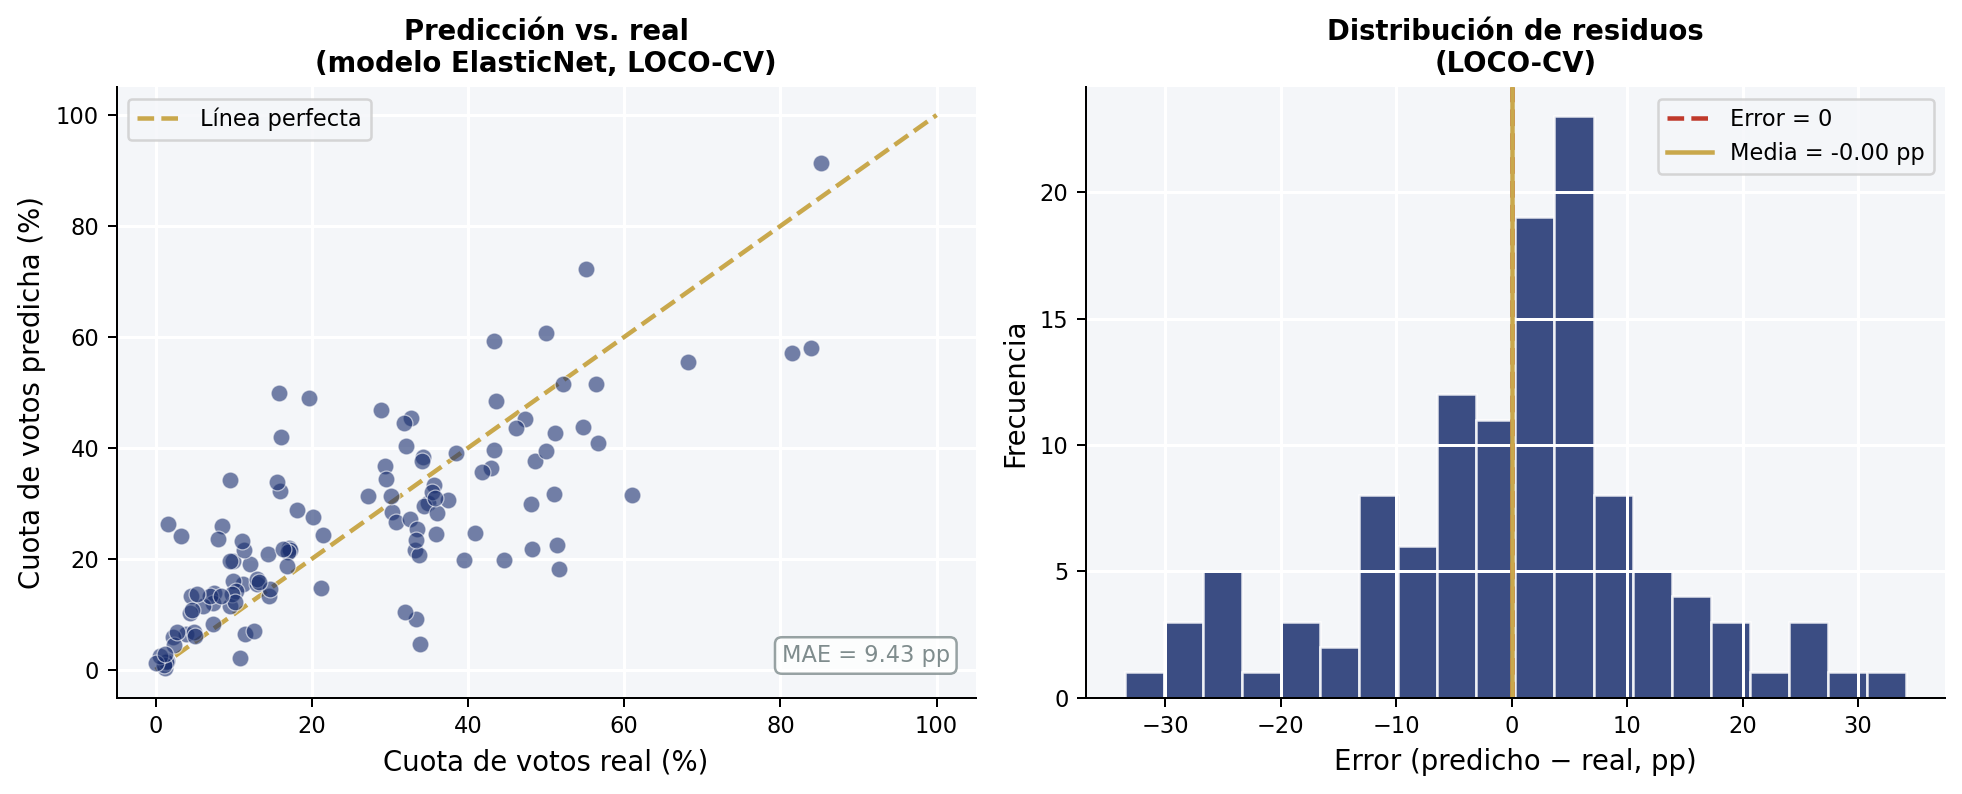
\includegraphics[width=0.85\textwidth]{img/colombia/col_loco_residuals.png}
  \end{center}
  \vspace{-0.4em}
  \begin{tikzpicture}
    \fill[elanPanel] (0,0) rectangle (\textwidth,0.75);
    \node[anchor=west, xshift=0.3cm, yshift=0.37cm] at (0,0)
      {{\color{elanGold}\small\bfseries MAE~=~9.43~pp} \quad
       {\color{elanGray}\small $\cdot$ $R^2_{\text{oos}} = 0.518$ $\cdot$ Top-1 = 64.5\% (20/31) $\cdot$ sin patrones sistem\'aticos de sesgo}};
  \end{tikzpicture}
\end{frame}

}% fin \etapacolombia
